% draft settings
\documentclass[letterpaper,12pt]{article}
\usepackage[margin=0.75in]{geometry}
\usepackage{setspace}

% **************************************************************
% figure management
\usepackage{graphicx}
\usepackage[labelfont=bf]{caption}

% table management
\usepackage{rotating}
\usepackage{booktabs}

% bib management
\usepackage[hidelinks]{hyperref}
\usepackage[numbers]{natbib}
\bibliographystyle{nar}

% font management
\usepackage[T1]{fontenc}
\usepackage[utf8]{inputenc}
\usepackage{microtype}

% misc
\usepackage{url}
\usepackage{lipsum}

% **************************************************************

% Include Supplement in the paper (resets all counters)
\newcommand{\beginsupplement}{%
        \setcounter{table}{0}
        \renewcommand{\thetable}{S\arabic{table}}%
        \setcounter{figure}{0}
        \renewcommand{\thefigure}{S\arabic{figure}}%
     }

% **************************************************************

\begin{document}
\beginsupplement

\title{Supplementary Information}
\maketitle

\begin{figure*}[!ht]
\centering
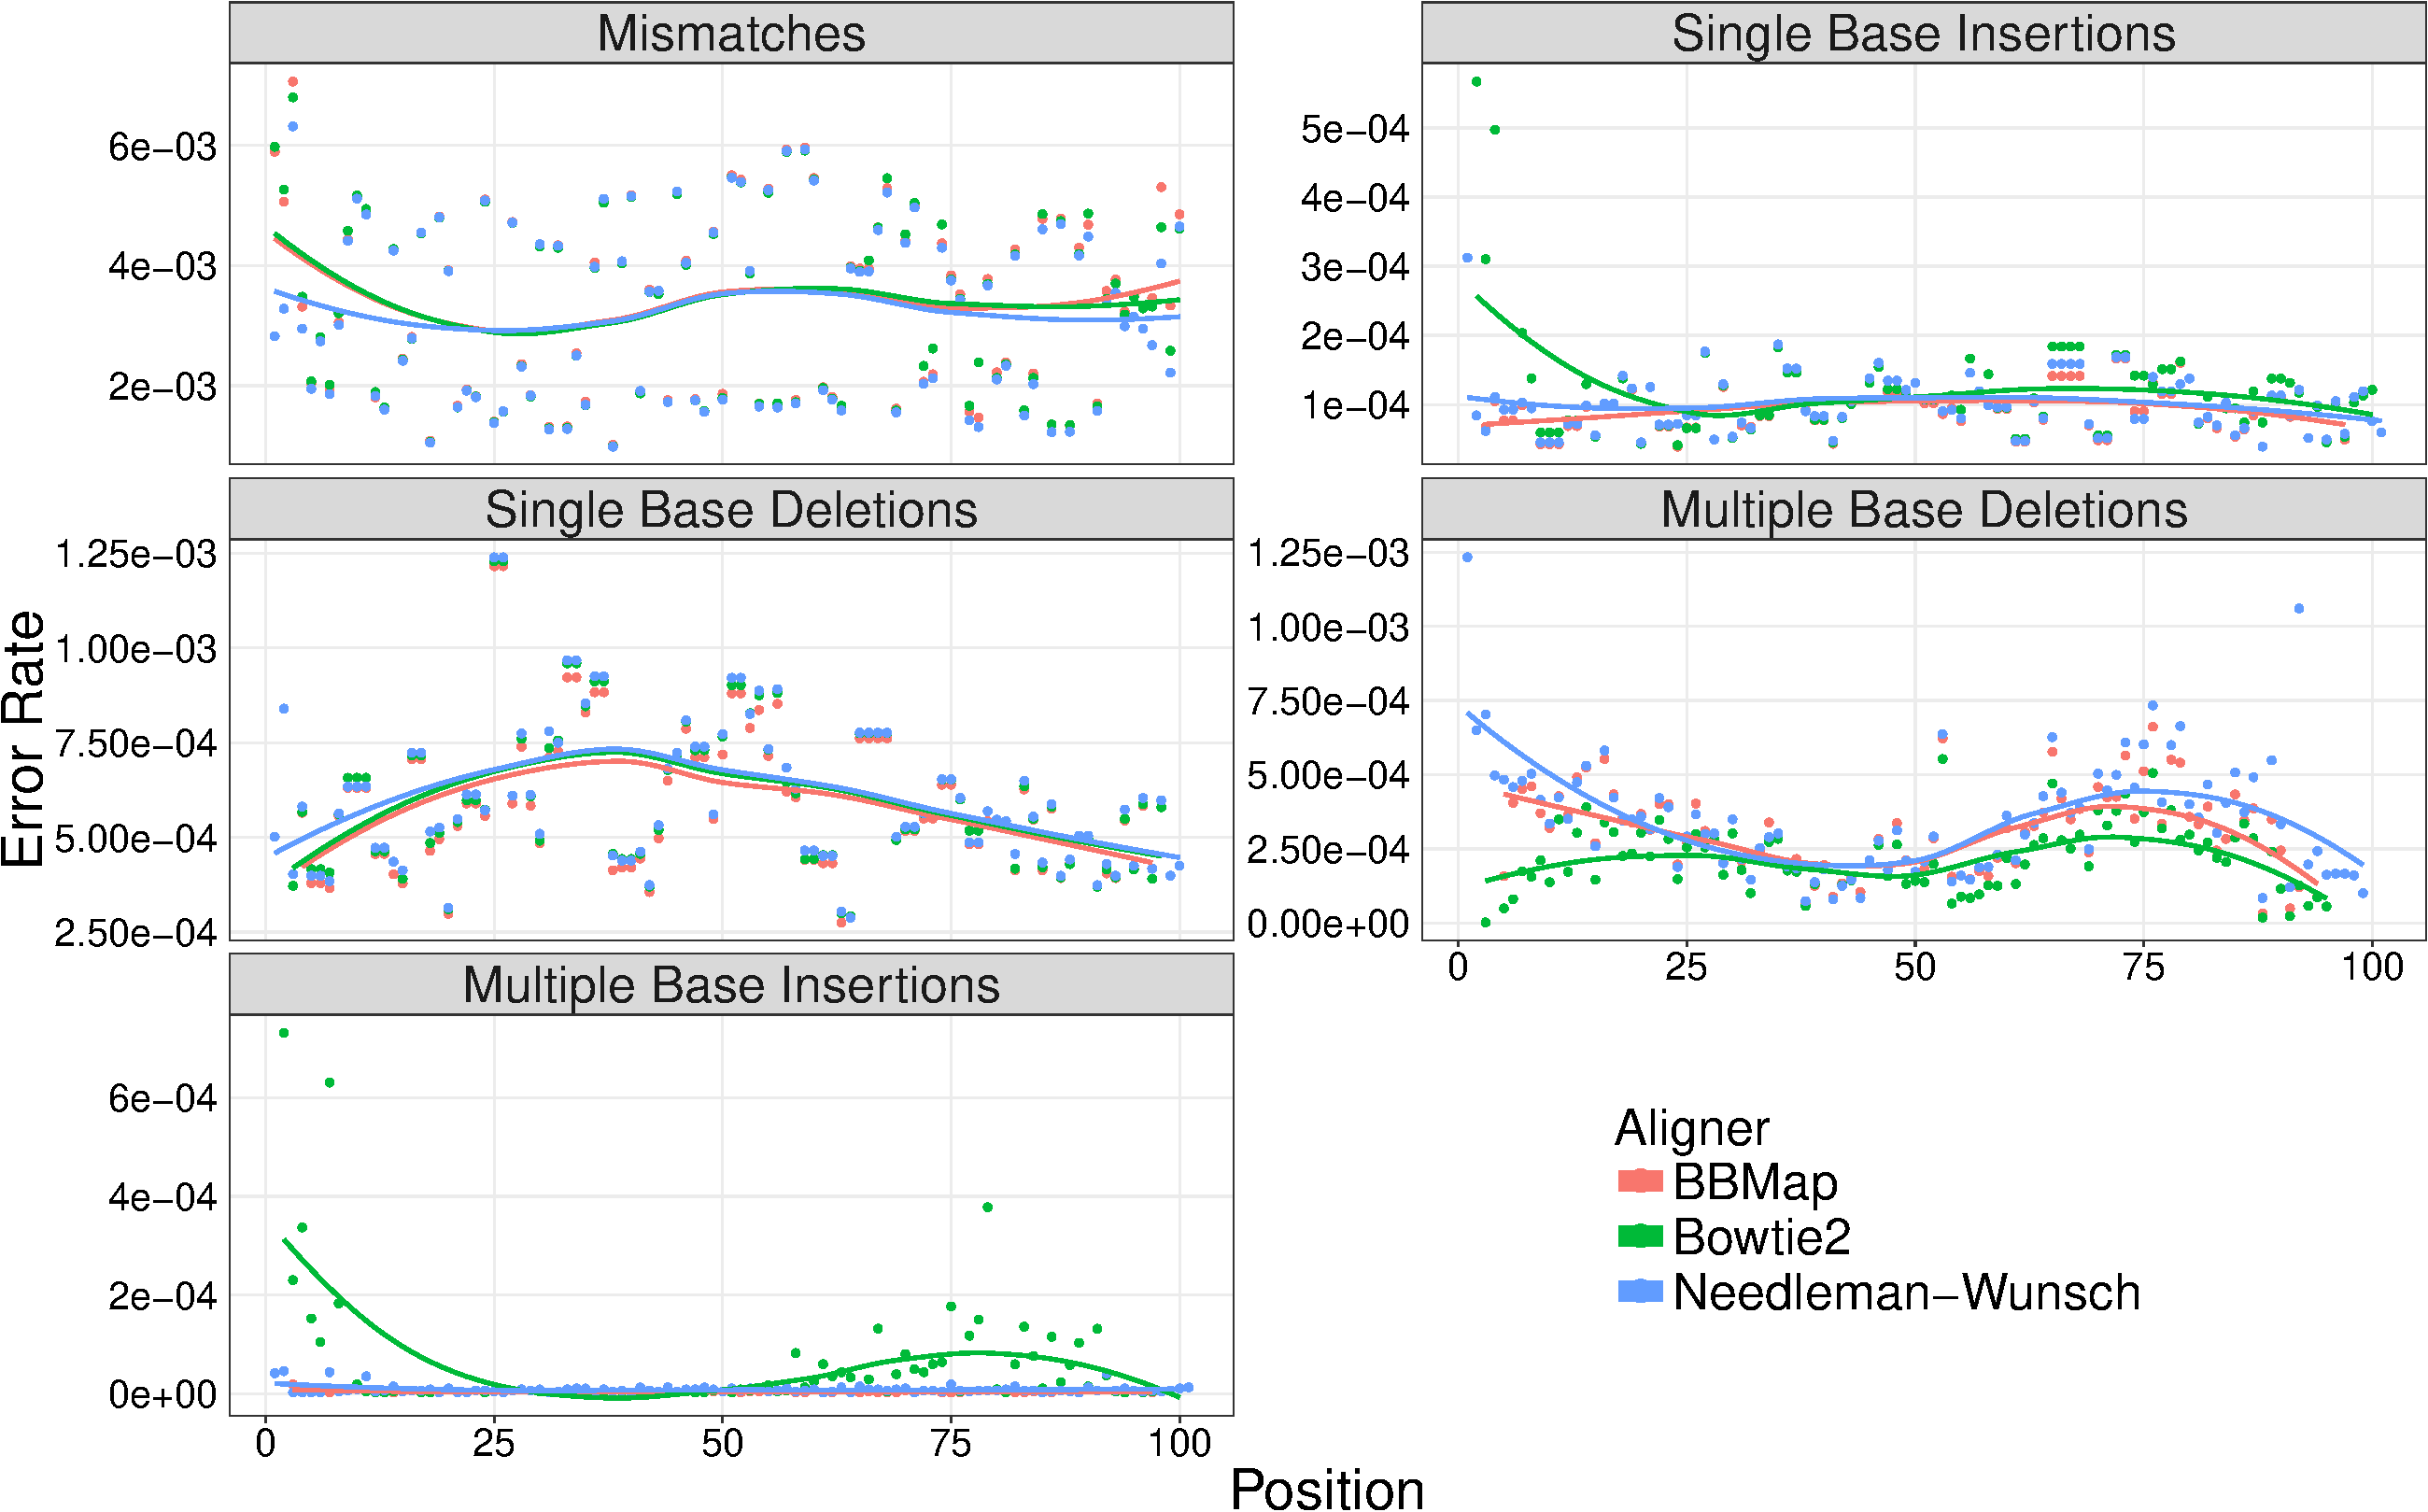
\includegraphics[width=174mm]{aligners-1.pdf}
\caption{\small \textbf{Effect of read aligner on error rates.} Here we mapped reads from the standard IDT oligo with \texttt{BBMap} (red), \texttt{Bowtie2} (green), and our Needleman-Wunsch aligner (blue), and quantified the error rates with our pipeline. We see that the choice of aligner affects the resulting error rates, especially for detecting multiple-base deletions.}
\end{figure*}

\clearpage
\begin{figure*}[t]
\centering
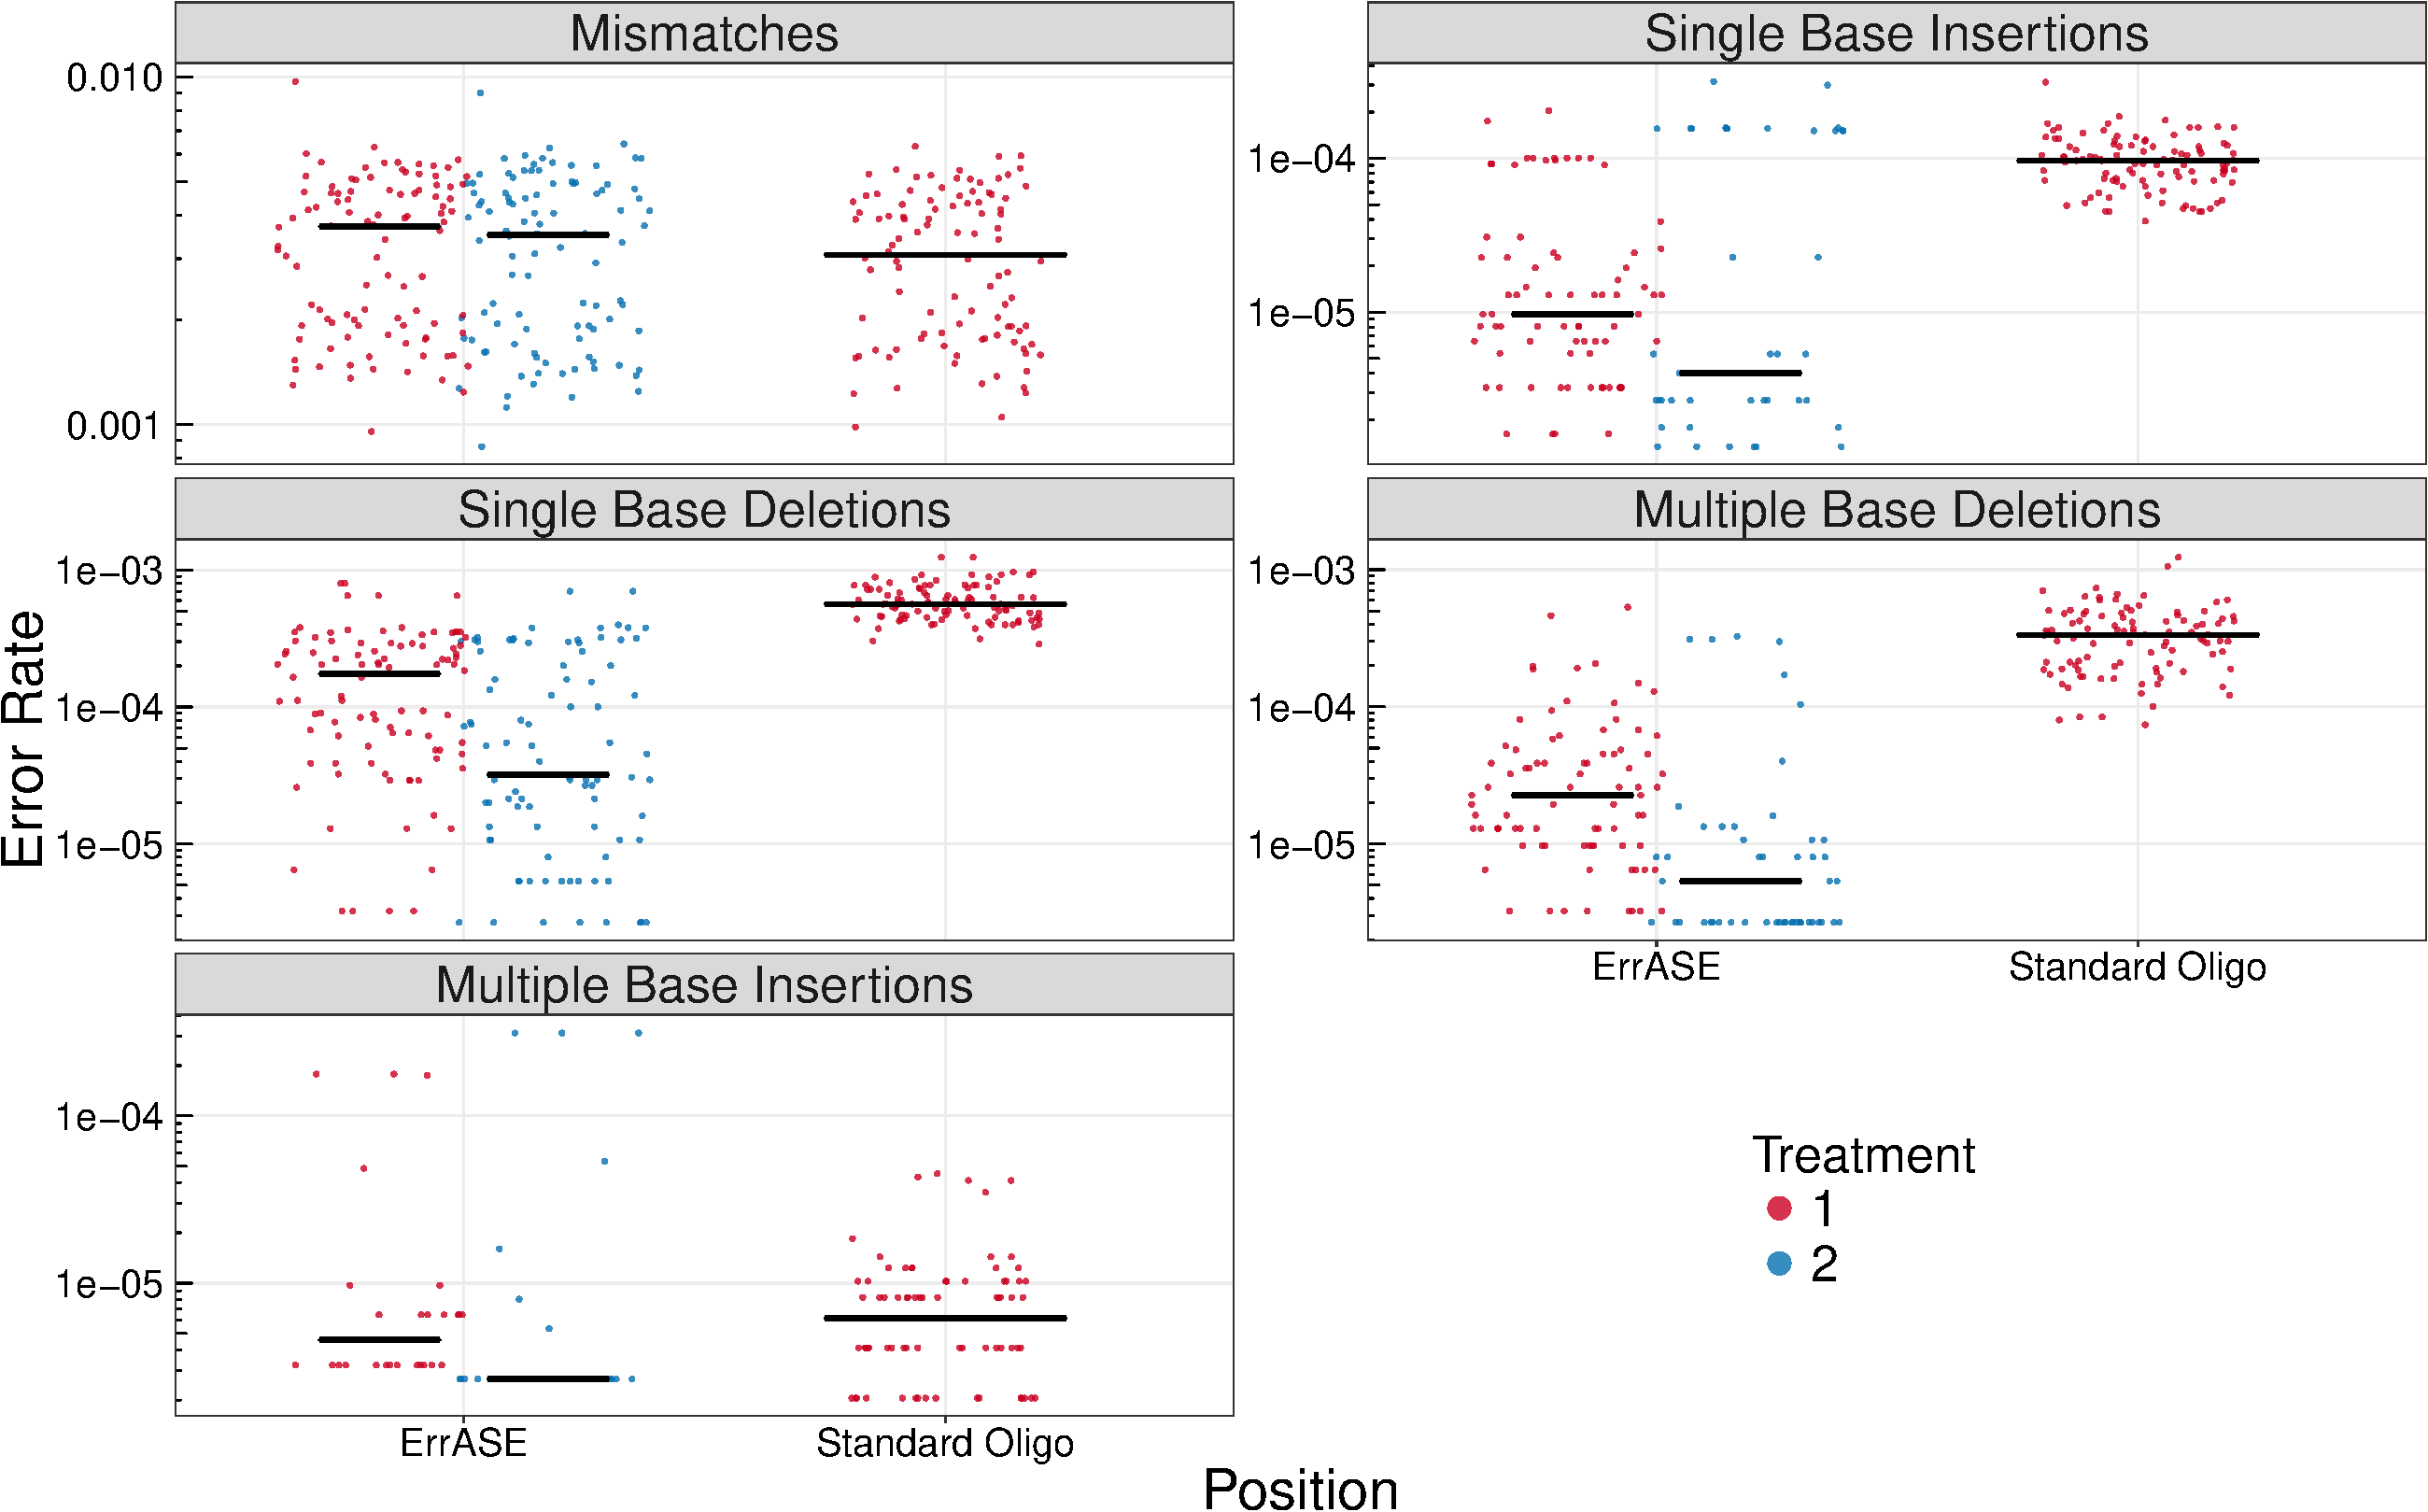
\includegraphics[width=174mm]{nonDoped_vs_ErrASE-1.pdf}
\caption{\small \textbf{Distributions of error rates per position for the standard oligo assembly before and after ErrASE treatment.} We were unable to detect a significant change between the median error rate after two treatments for mismatches. \textbf{Note:} black bar is median value.}
\end{figure*}

\clearpage
\begin{figure*}[t]
\centering
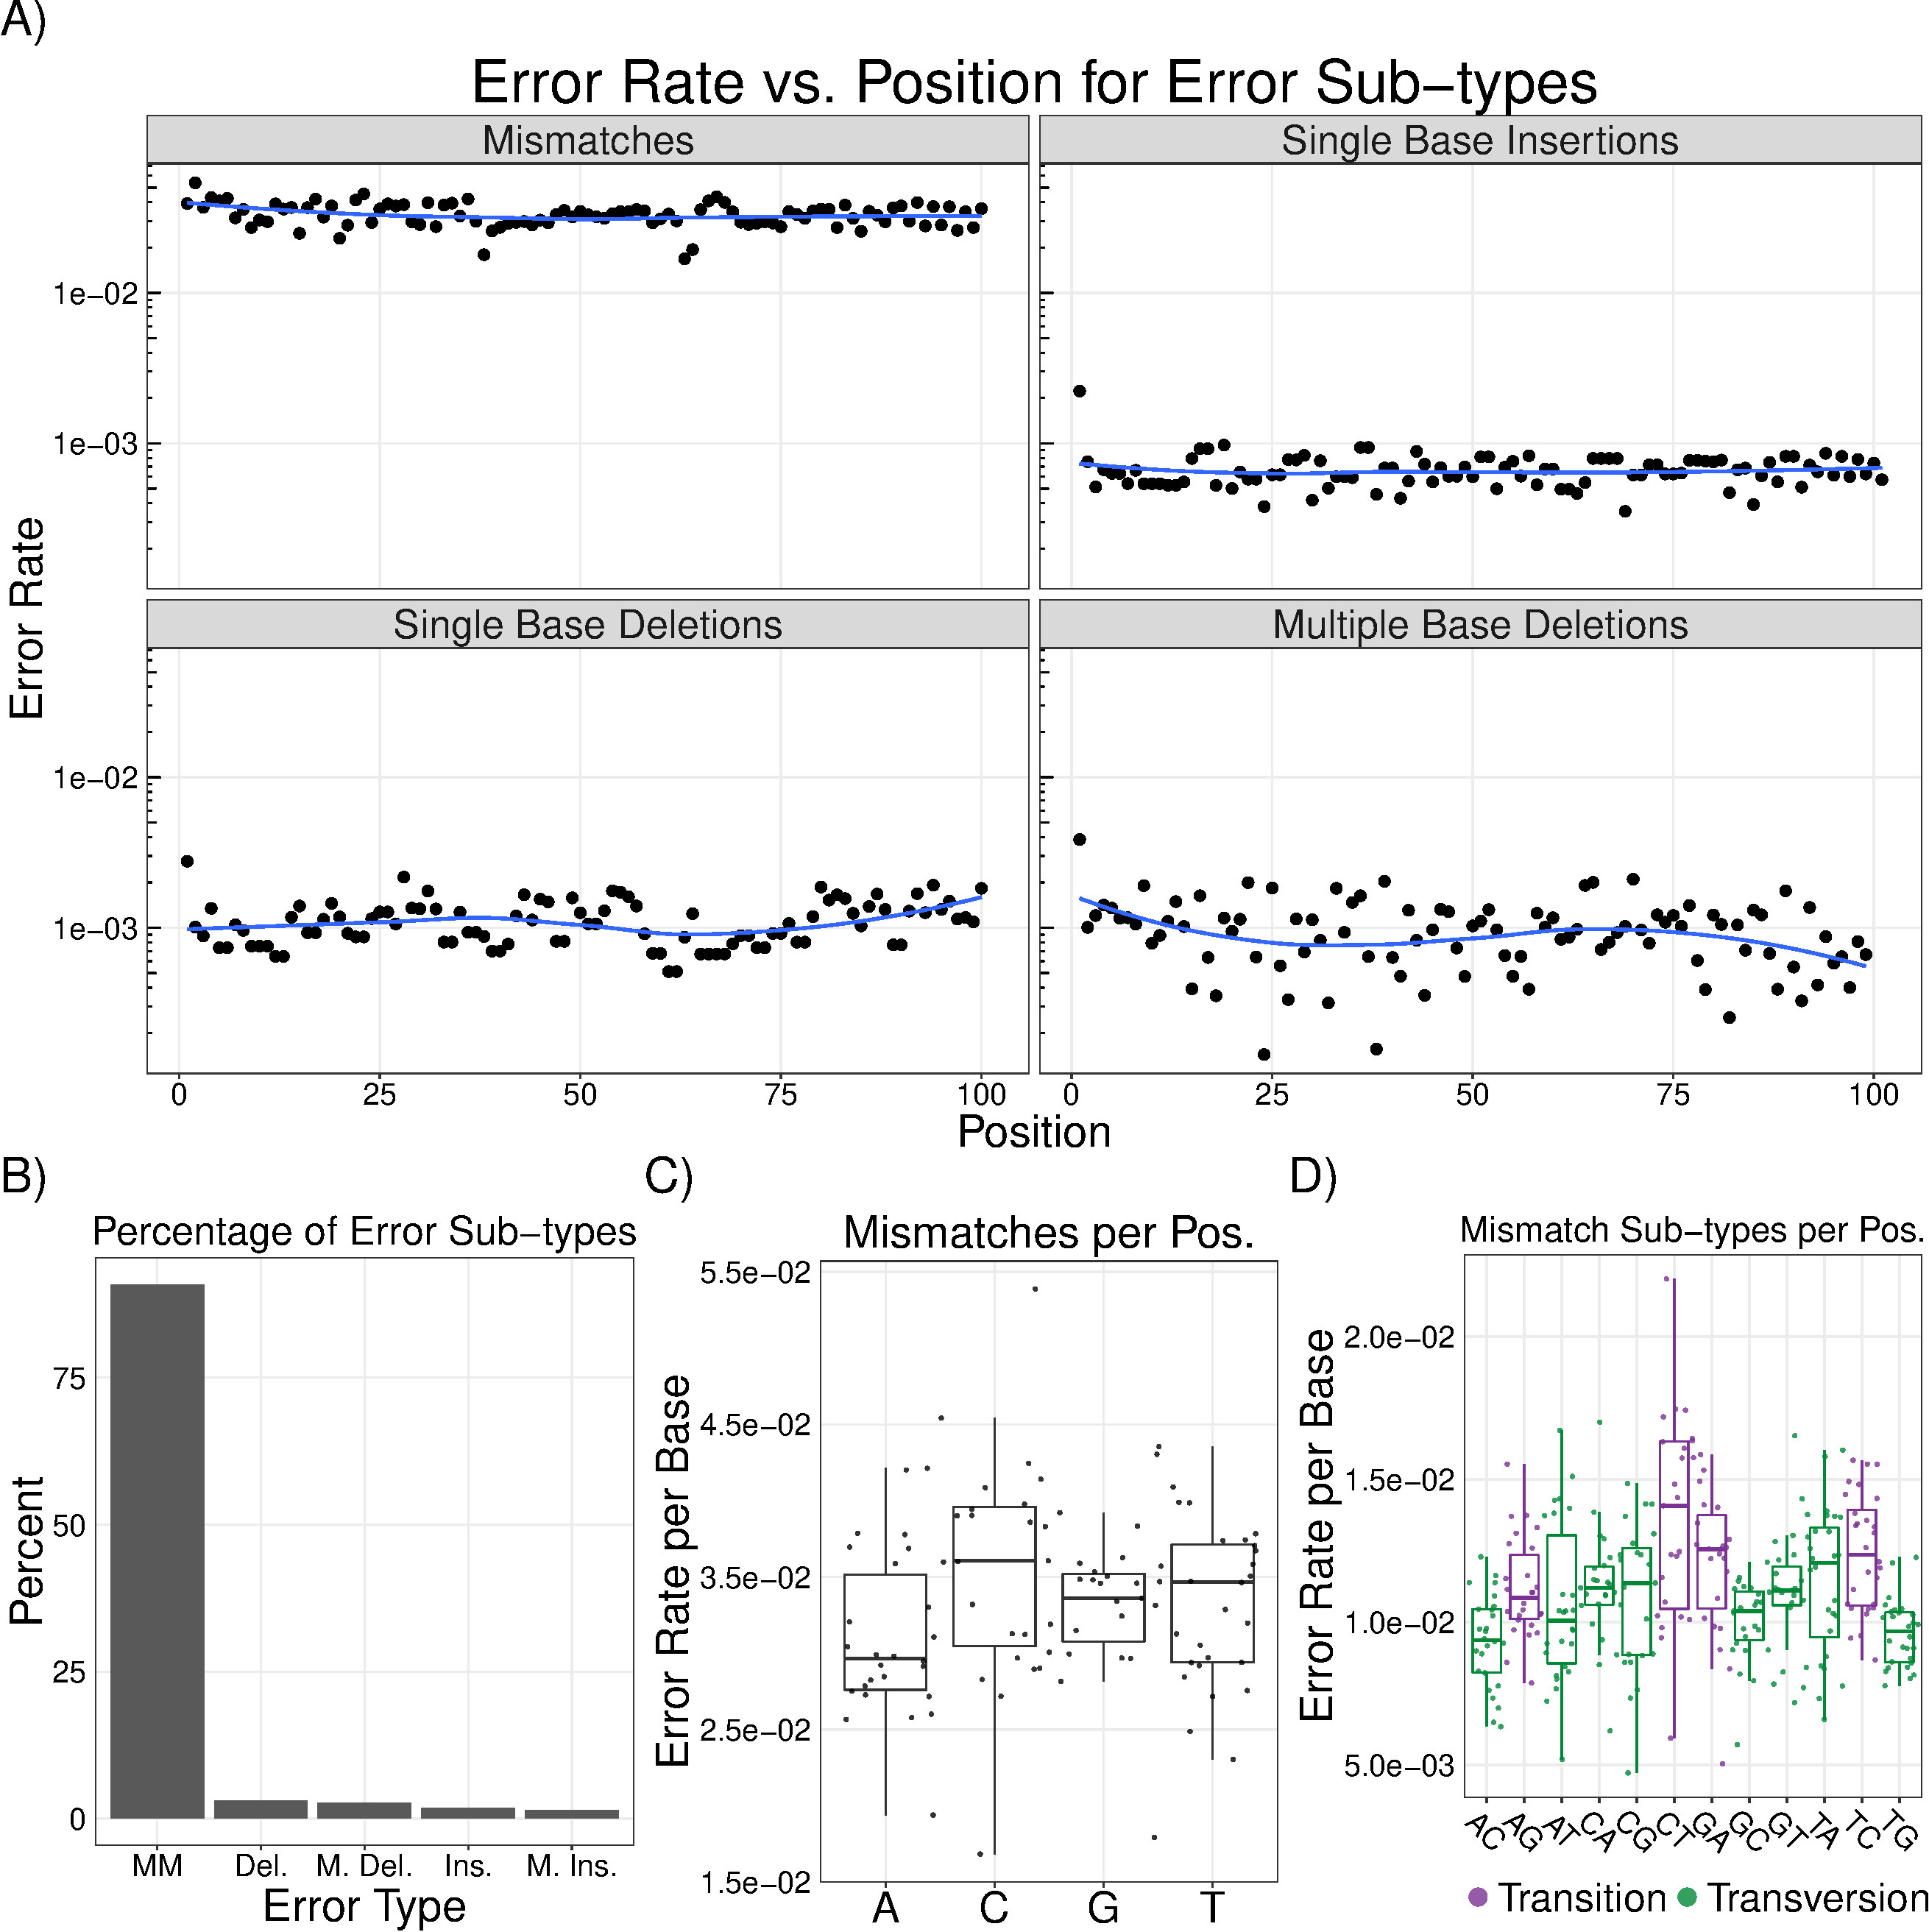
\includegraphics[width=174mm]{doped_analysis-1.pdf}
\caption{\small \textbf{In-depth analysis of error-doped assemblies.} Here, we find no significant difference in the median mismatch rate of all four bases, median transition or transversion rate, or rate of single-base deletions for each base (all tests were Mann-Whitney U, NS, Holm-corrected). \textbf{Note:} here we performed the same analysis as Figure 2 in the main text with the error-doped assembly.}
\end{figure*}

\clearpage
\begin{figure*}[t]
\centering
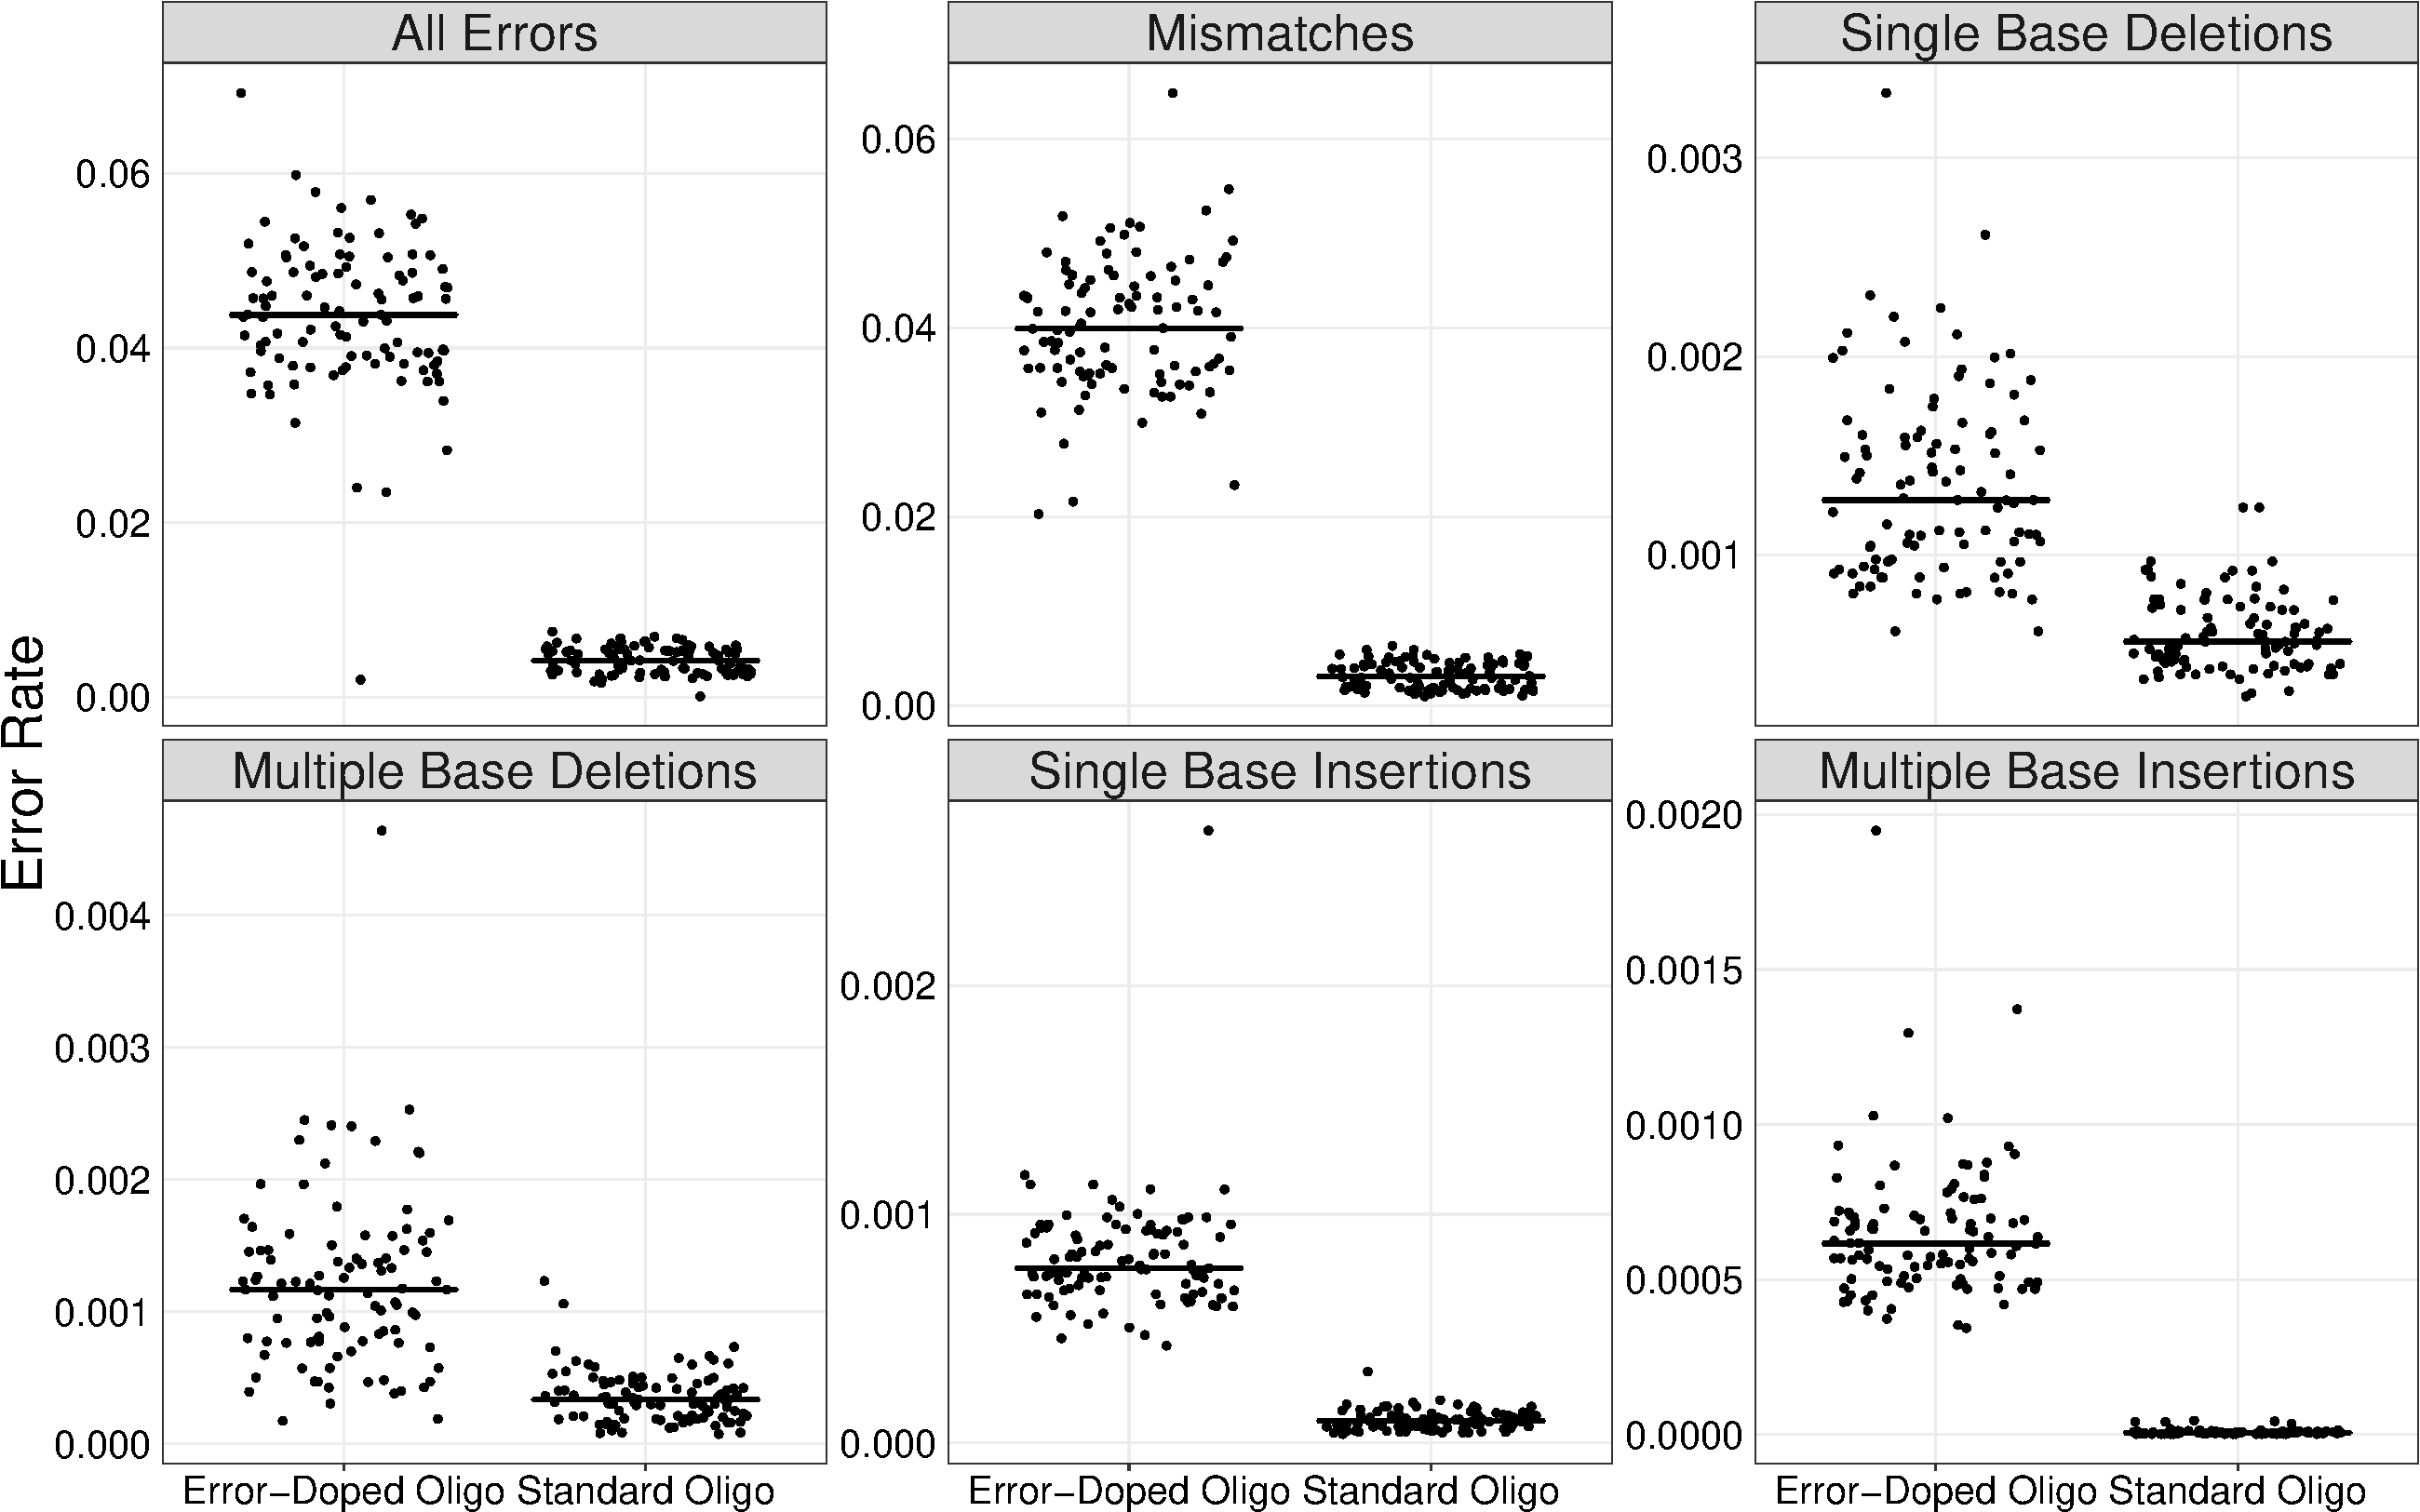
\includegraphics[width=174mm]{Dope_vs_NonDope-1.pdf}
\caption{\small \textbf{Comparison of measured error rates from error-doped and standard oligos.} Here we plot the distribution of error rates per position and see that for every error sub-type the error rates are significantly higher for the error-doped oligos than those produced by the standard process (Mann-Whitney U Test, all $p << 0.001$). \textbf{Note:} Black bar is the median value.}
\end{figure*}

\clearpage
\begin{figure*}[t]
\centering
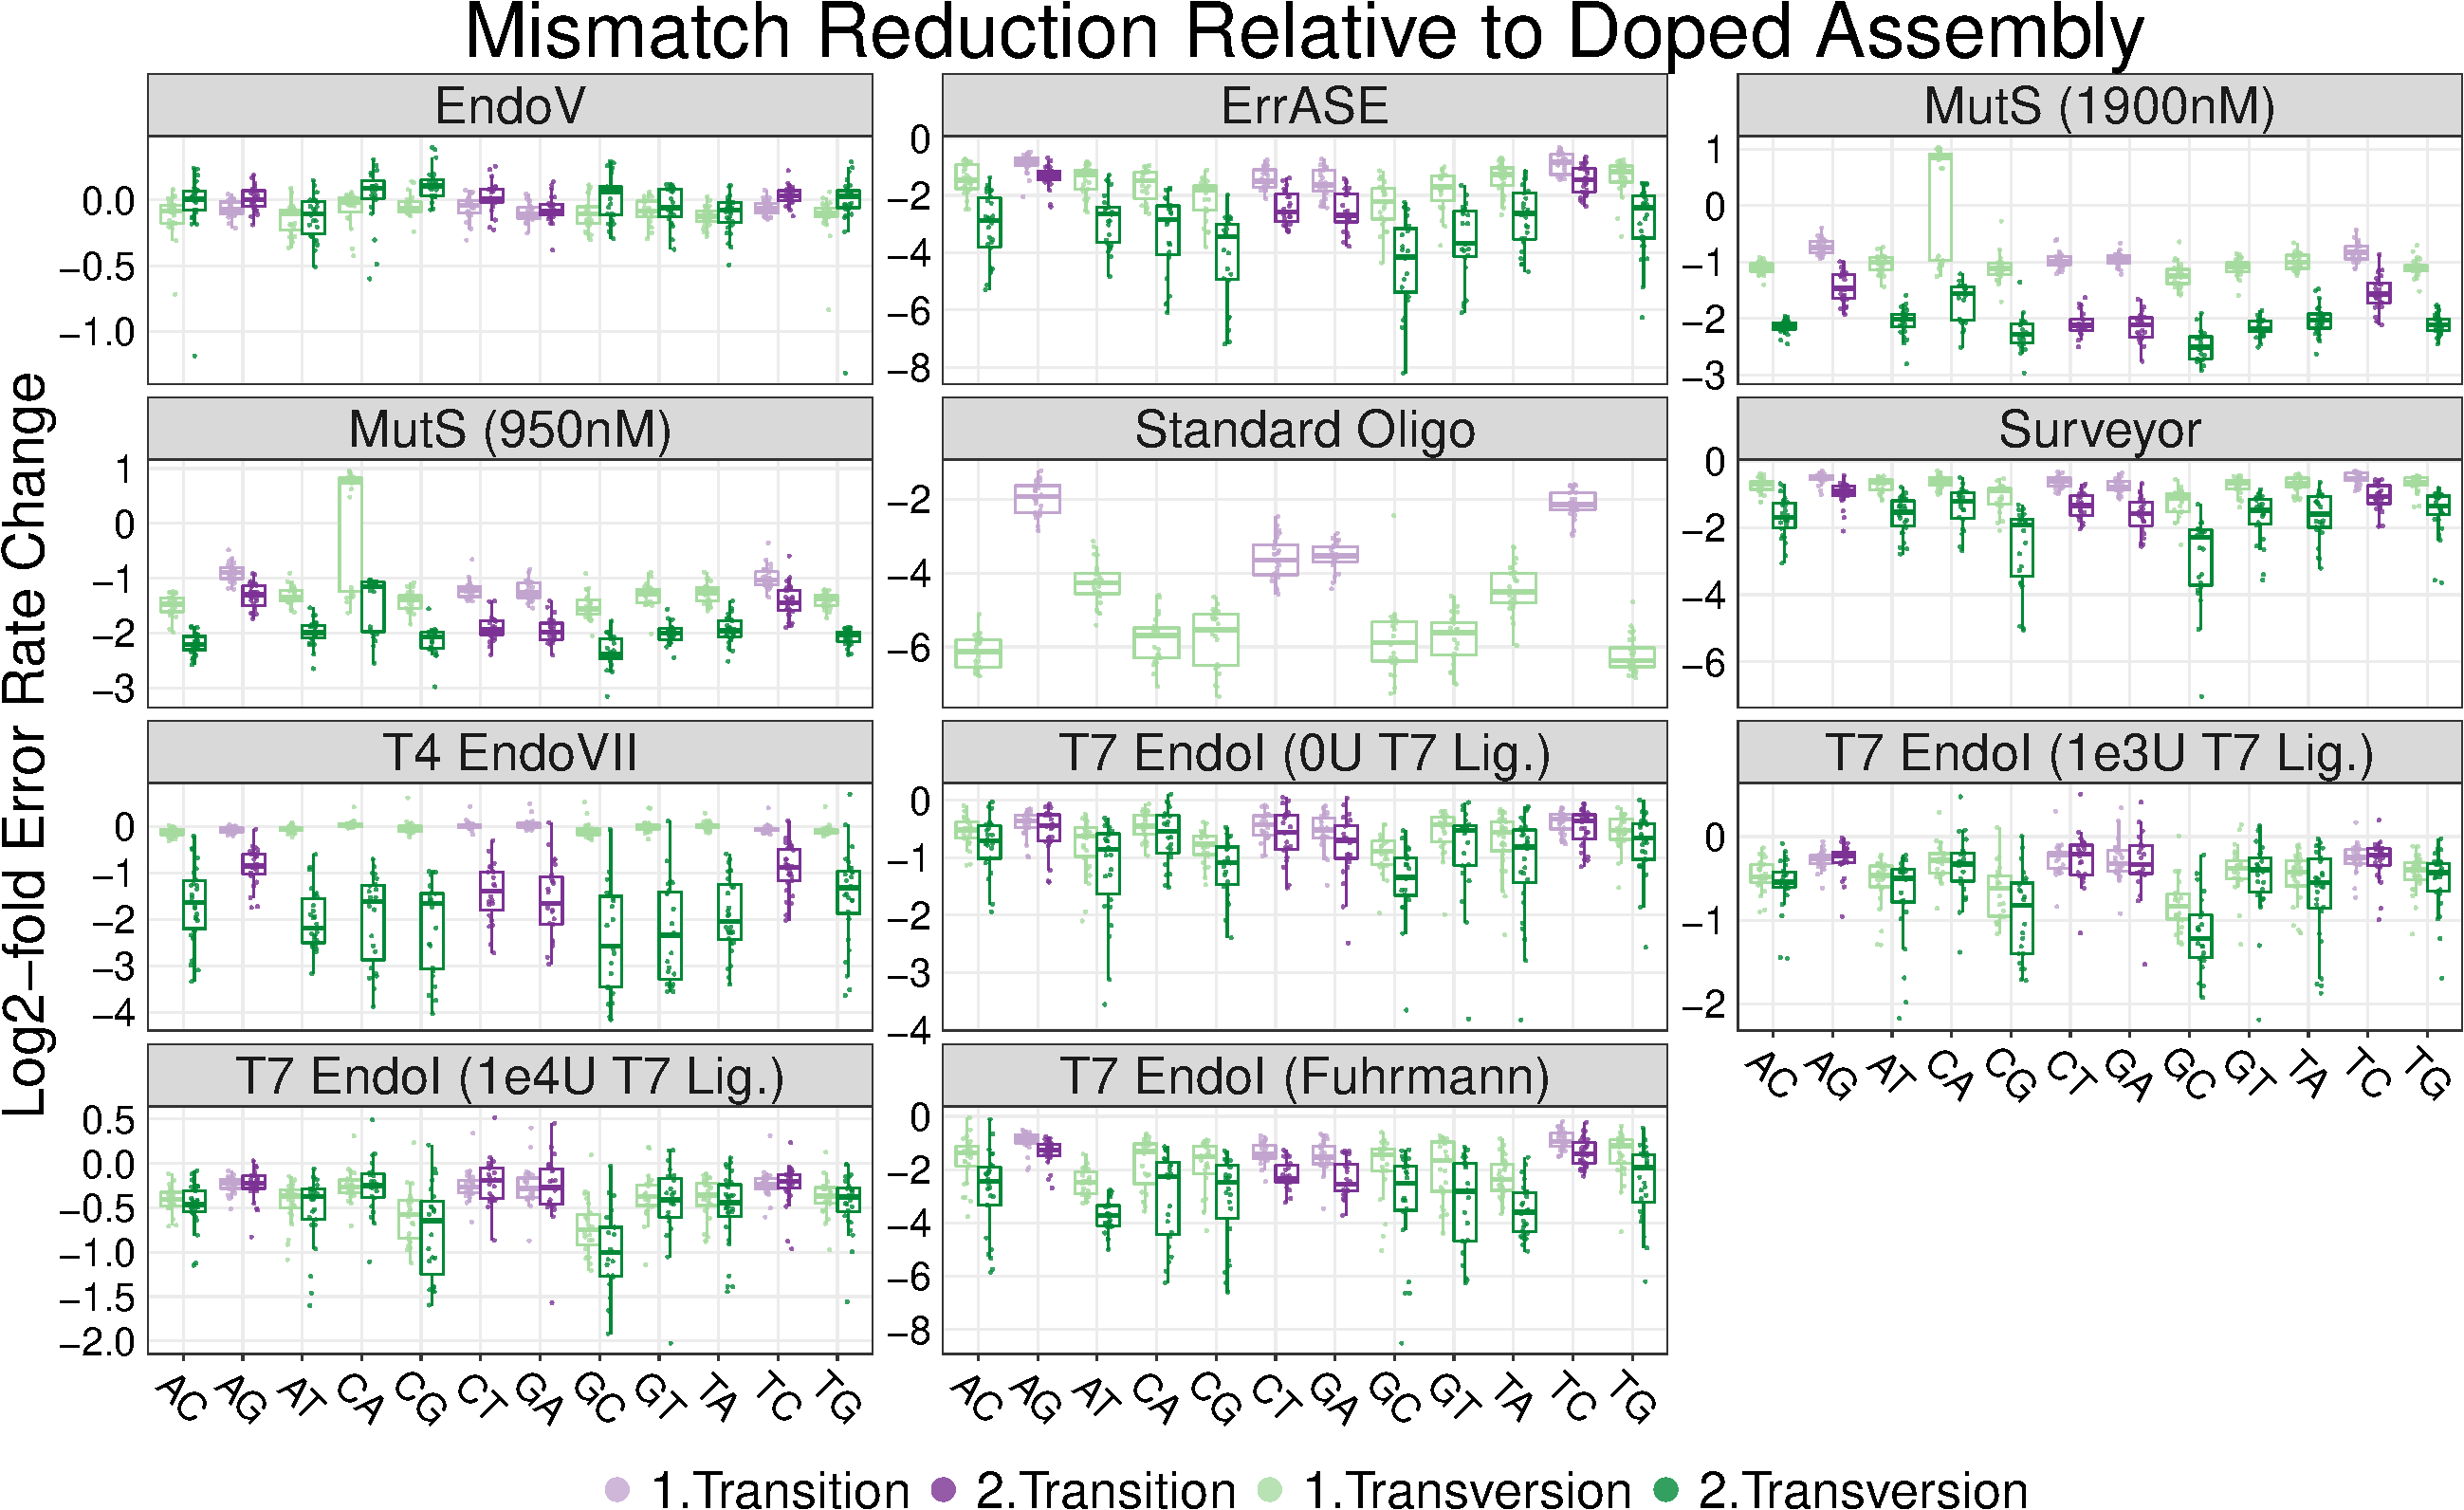
\includegraphics[width=174mm]{Enzyme_Prefs_MM-1.pdf}
\caption{\small \textbf{Mismatch correction preferences relative to the error-doped oligo for every enzyme across two consecutive treatments.} Error rates are plotted as the $\log_2$-fold-change in error rate relative to the error-doped template. \textbf{Note:} box plots are first and third quartile for hinges, median for bar, and $1.5\times$ the inter-quartile range for whiskers.}
\end{figure*}

\clearpage
\begin{figure*}[t]
\centering
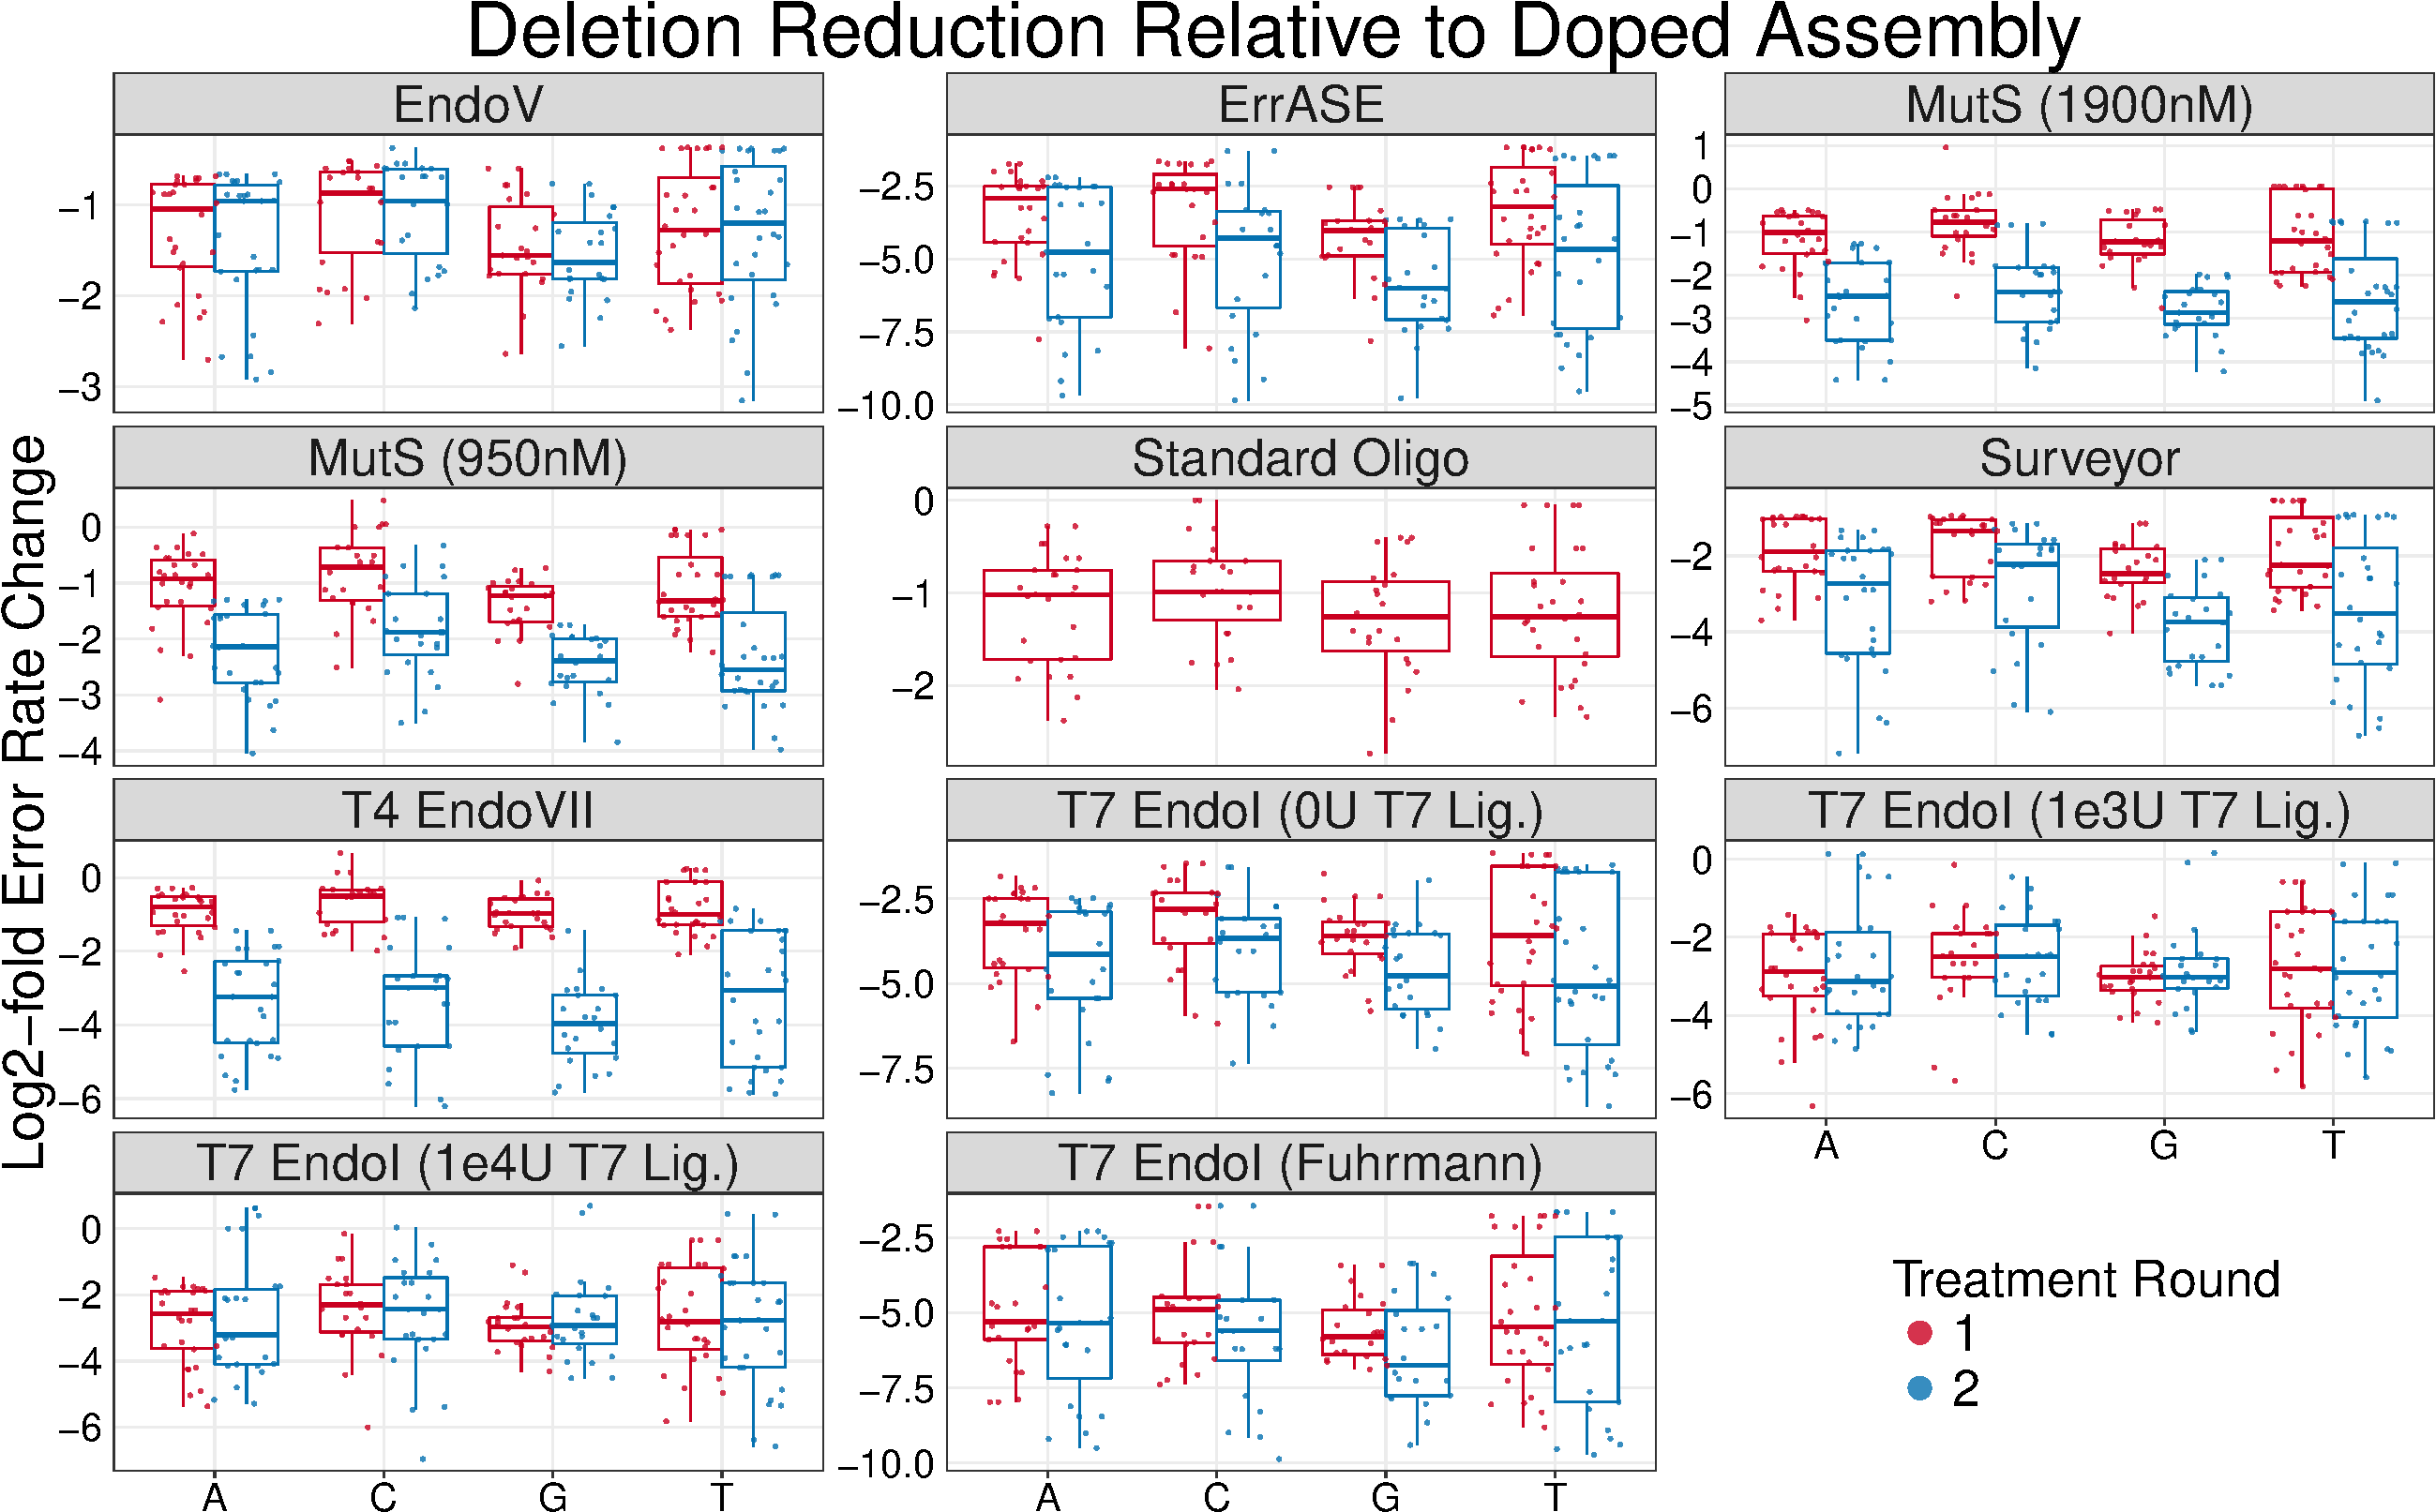
\includegraphics[width=174mm]{Enzyme_Prefs_Deletions-1.pdf}
\caption{\small \textbf{Single-base deletion correction preferences relative to the error-doped oligo for every enzyme across two consecutive treatments.} Error rates are plotted as the $\log_2$-fold-change in error rate relative to the error-doped template. \textbf{Note:} box plots are first and third quartile for hinges, median for bar, and $1.5\times$ the inter-quartile range for whiskers.}
\end{figure*}

\clearpage
\begin{figure*}[t]
\centering
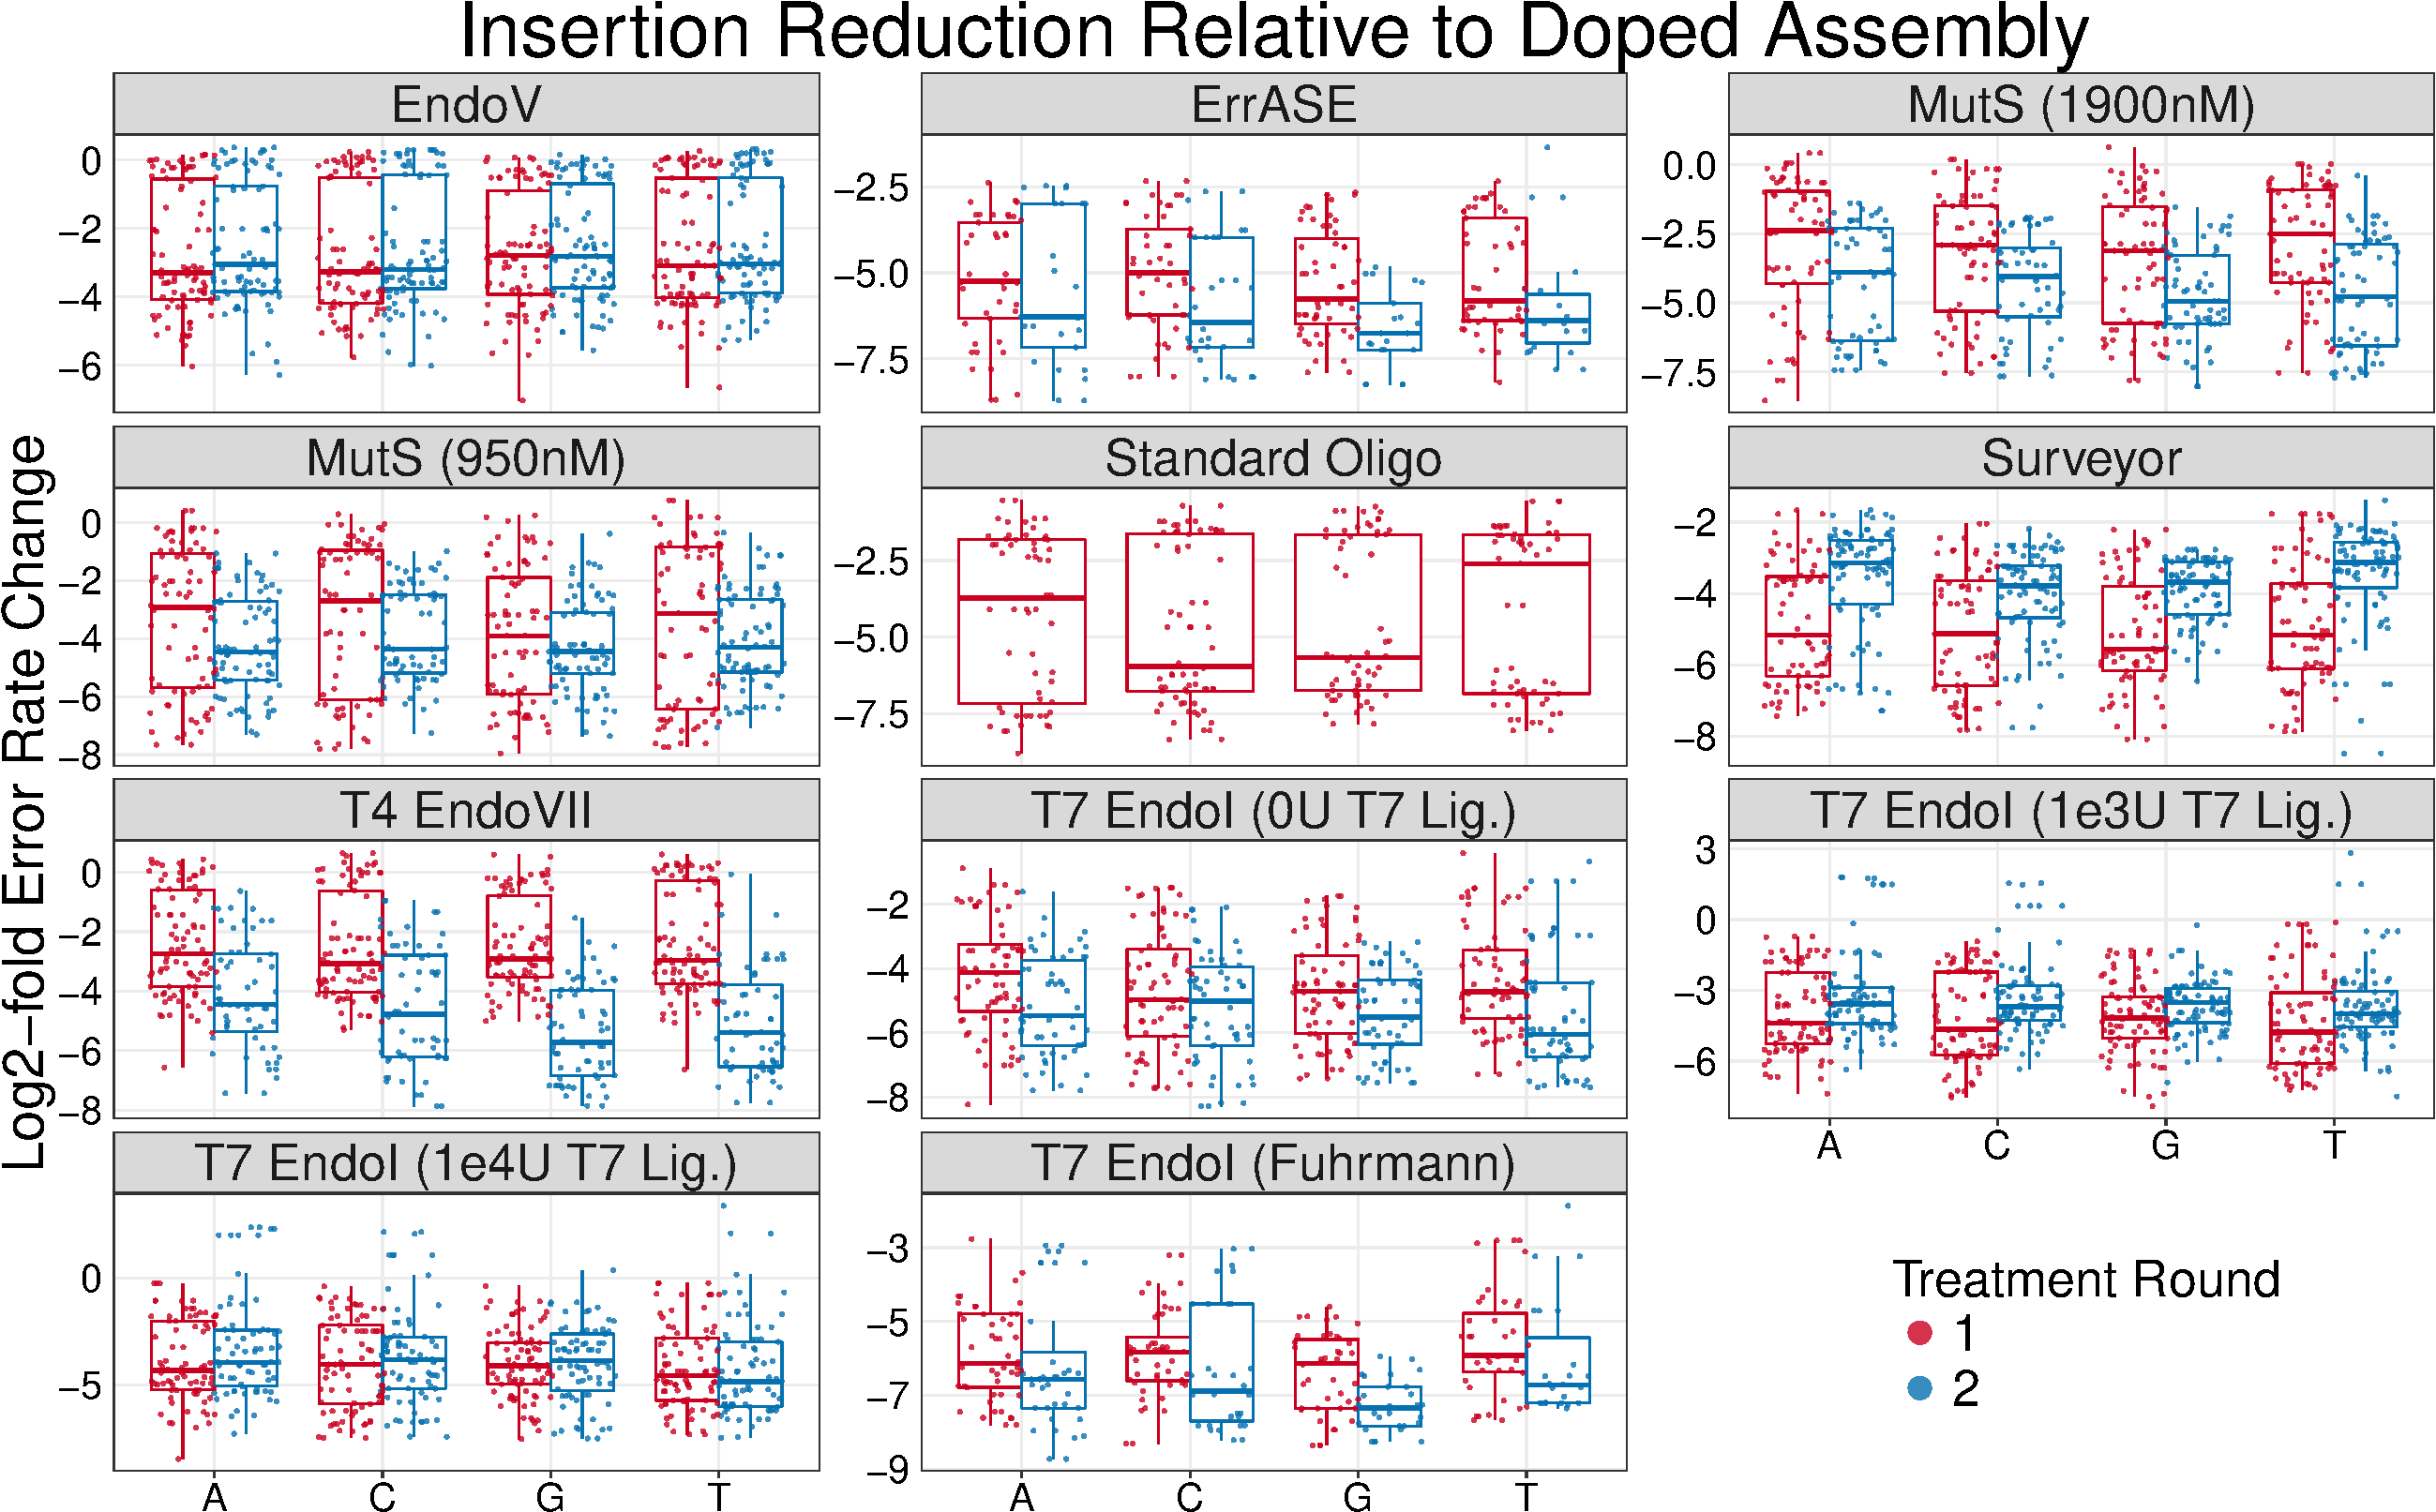
\includegraphics[width=174mm]{Enzyme_Prefs_Insertions-1.pdf}
\caption{\small \textbf{Single-base insertion correction preferences relative to the error-doped oligo for every enzyme across two consecutive treatments.} Error rates are plotted as the $\log_2$-fold-change in error rate relative to the error-doped template. \textbf{Note:} box plots are first and third quartile for hinges, median for bar, and $1.5\times$ the inter-quartile range for whiskers.}
\end{figure*}

\clearpage
\begin{sidewaystable*}[!t]
\centering
\caption{\textbf{Examples of where various aligners fail.} Here \texttt{\_} are padding for visualization, \texttt{*} are soft-trimming, and lower-case bases are inserts.}
\texttt{
\begin{tabular}{@{}lllll@{}}
\toprule
\textbf{Aligner:} & \textbf{Ideal}          & \textbf{Needleman-Wunsch} & \textbf{Bowtie2}         & \textbf{BBMap}         \\ \midrule
Reference: & \_GCTGCCGATTTCCA...    & \_GCTGCCGATTTCCA...    & G\_CTGCCGATTTCCA...      & *GCTGCCGATTTCCA...     \\
Read:      & aGCTGCCGATTTCCA...     & aGCTGCCGATTTCCA...     & aGCTGCCGATTTCCA...       & *GCTGCCGATTTCCA...     \\ \midrule
Reference: & \_\_GCTGCCGATTTCCA...  & \_\_GCTGCCGATTTCCA...  & G\_\_CTGCCGATTTCCA...    & **GCTGCCGATTTCCA...    \\
Read:      & aaGCTGCCGATTTCCA...    & aaGCTGCCGATTTCCA...    & aaGCTGCCGATTTCCA...      & **GCTGCCGATTTCCA...    \\ \midrule
Reference: & GCTGCCGATTTCCA...      & GCTGCCGATTTCCA...      & GCTGCCGATTTCCA...        & GCTGCCGATTTCCA...      \\
Read:      & GCT\_\_\_GATTTCCA...   & GCT\_\_\_GATTTCCA...   & \_\_\_GCTGATTTCCA...     & \_\_\_GCTGATTTCCA...   \\ \midrule
Reference: & GCTGCCGATTTCCA...      & GCTGCCGATTTCCA...      & GCTGCCGAT\_TTCCA...      & GCTGCCGATTTCCA...      \\
Read:      & GCTG\_\_\_\_\_TTCCA... & GCTG\_\_\_\_\_TTCCA... & \_\_\_\_\_\_GCTGTTCCA... & GCTG\_\_\_\_\_TTCCA... \\ \midrule
Reference: & ...TGTTGTATATATCG\_    & ...TGTTGTATATATCG\_    & ...TGTTGTATATATC\_G      & ...TGTTGTATATATCG*     \\
Read:      & ...TGTTGTATATATCGa     & ...TGTTGTATATATCGa     & ...TGTTGTATATATCaG       & ...TGTTGTATATATCG*     \\ \midrule
Reference: & ...TGTTGTATATATC\_\_G  & ...TGTTGTATATATC\_\_G  & ...TGTTGTATATATC\_\_G    & ...TGTTGTATATATCG**    \\
Read:      & ...TGTTGTATATATCatG    & ...TGTTGTATATATCatG    & ...TGTTGTATATATCatG      & ...TGTTGTATATATCa**    \\ \midrule
Reference: & ...TGTTGTATATAT\_\_CG  & ...TGTTGTATATA\_\_TCG  & ...TGTTGTATATA\_\_TCG    & ...TGTTGTATATATCG**    \\
Read:      & ...TGTTGTATATATgtCG    & ...TGTTGTATATATgtCG    & ...TGTTGTATATATgtCG      & ...TGTTGTATATATgt**    \\ \midrule
Reference: & ...TGTTGTATATATCG      & ...TGTTGTATATATCG      & ...TGTTGTATATATCG        & ...TGTTGTATATATCG      \\
Read:      & ...TGTTGTATATA\_\_G    & ...TGTTGTATATA\_\_G    & ...TGTTGTATATAG\_\_      & ...TGTTGTATATAG\_\_    \\ \midrule
Reference: & ...TGTTGTATATAT\_\_CG  & ...TGTTGTATATA\_\_TCG  & ...TGTTGTATATA\_\_TCG    & ...TGTTGTATATATCG**    \\
Read:      & ...TGTTGTATATATgtCG    & ...TGTTGTATATATgtCG    & ...TGTTGTATATATgtCG      & ...TGTTGTATATATgt**    \\ \bottomrule
\end{tabular}
}
\end{sidewaystable*}

\end{document}

